%Dave's handout 6.3 Definite Integrals and Area

\vspace{-0.25 in}
\begin{framed}
\subsection*{Objectives}
\begin{itemize}
    \item Understand the use of definite integrals to determine the area of a region bounded by the x-axis and the graph of a function.
\end{itemize}

%%%Reading Assignment%%%
\subsection*{Suggested Reading:}
\begin{itemize}
\item \cite{Calaway}\footnotemark[1]
   \begin{itemize}
        \item \emph{Section 3.1 The Definite Integral}
        \begin{itemize}
            \item Approximating with Rectangles
            \item Definition of the Definite Integral
            \item \emph{Signed Area}
        \end{itemize}
    \end{itemize}
\item \cite{openstax}\footnotemark[2]\textsuperscript{,}\footnotemark[3]
    \begin{itemize}
        \item \emph{Section 5.2 The Definite Integral}
        \begin{itemize}
            \item Area and the Definite Integral
        \end{itemize}
    \end{itemize}
\end{itemize}
%\subsection*{Supplemental Materials:}
%%%Key Terms%%%
\subsection*{Key Terms and Concepts:} 


\begin{itemize}
    \item Area under the graph of a function; area as a limit of sum of areas of rectangles.
    \item Total Area vs. Net Signed Area
\end{itemize}

\end{framed}
\footnotetext[1]{Available free to download from \url{http://www.opentextbookstore.com/details.php?id=14} .}
\footnotetext[2]{Available free to download from \url{https://openstax.org/details/books/calculus-volume-1} .}
\footnotetext[3]{Disregard any examples with trigonometry.}

\newpage
%%%%%%%%%%START LESSON CONTENT%%%%%%%%%%%%%
%\noindent\makebox[\linewidth]{\rule{\textwidth}{0.8pt}}
\Opensolutionfile{ans}[ans22]
\Opensolutionfile{ansL}[ansL22]
%%%%%%%%%%%%%%%%Start First Topic%%%%%%%%%%%%%%%%%%%%%%%%%%%%%
\noindent Recall that the process of differentiation is used to provide a function, called the derivative, which is used to find the slope of a tangent line to the graph of the function.  It turns that the process of integration also provides information about the function being integrated. \\

%%%%%%%%%%%%%%Applied Calculus by Calaway%%%%%%%%%%%%%%%%%%%%%%%%%%
\begin{wrapfigure}[13]{r}{0.5\textwidth}

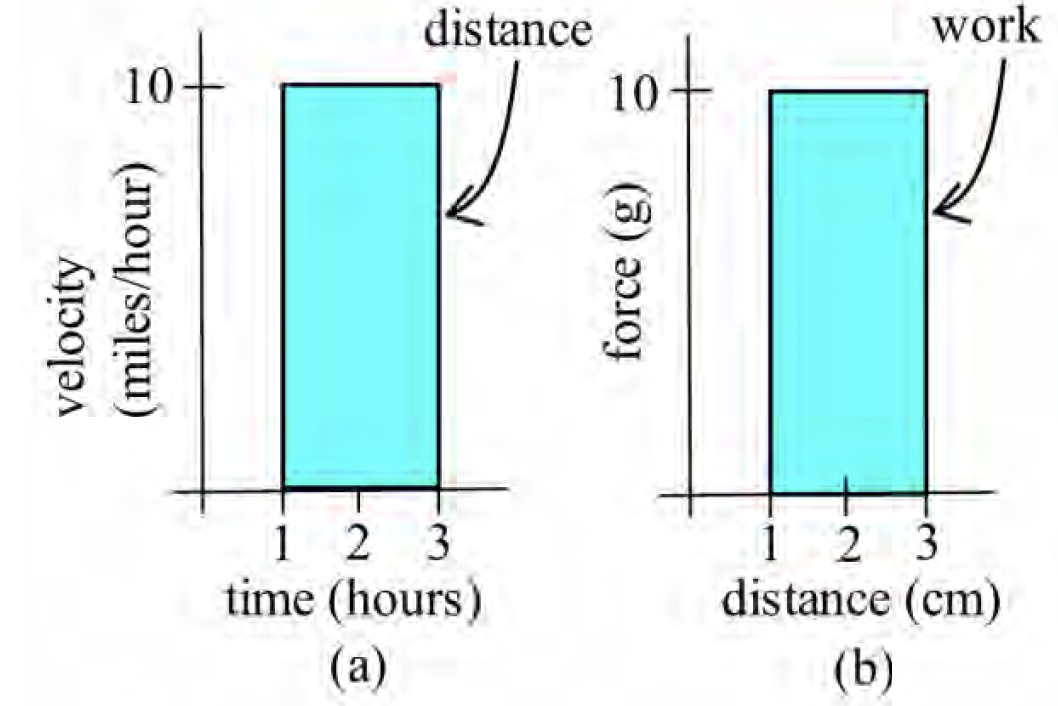
\includegraphics[scale=0.4]{images/defIntgArea/velocity_force.png}
\caption{ }
\label{fig:velocity_force}
\end{wrapfigure}

\noindent One reason areas are so useful is that they can represent quantities other than simple geometric shapes. If the units for each side of the rectangle are meters, then the area will have the units \emph{meters} $times$ \emph{meters} $=m^2$. But if the units of the base of a rectangle are hours and the units of the height are \emph{miles/hour}, then the units of the area of the rectangle are \emph{hours} $times$ \emph{miles/hour} = \emph{miles}, a measure of distance. Similarly, if the base units are \emph{centimeters} and the height units are \emph{grams}, then the area units are \emph{gram-centimeters}, a measure of work.\\
%\hfill \break

\begin{wrapfigure}[13]{l}{0.7\textwidth}
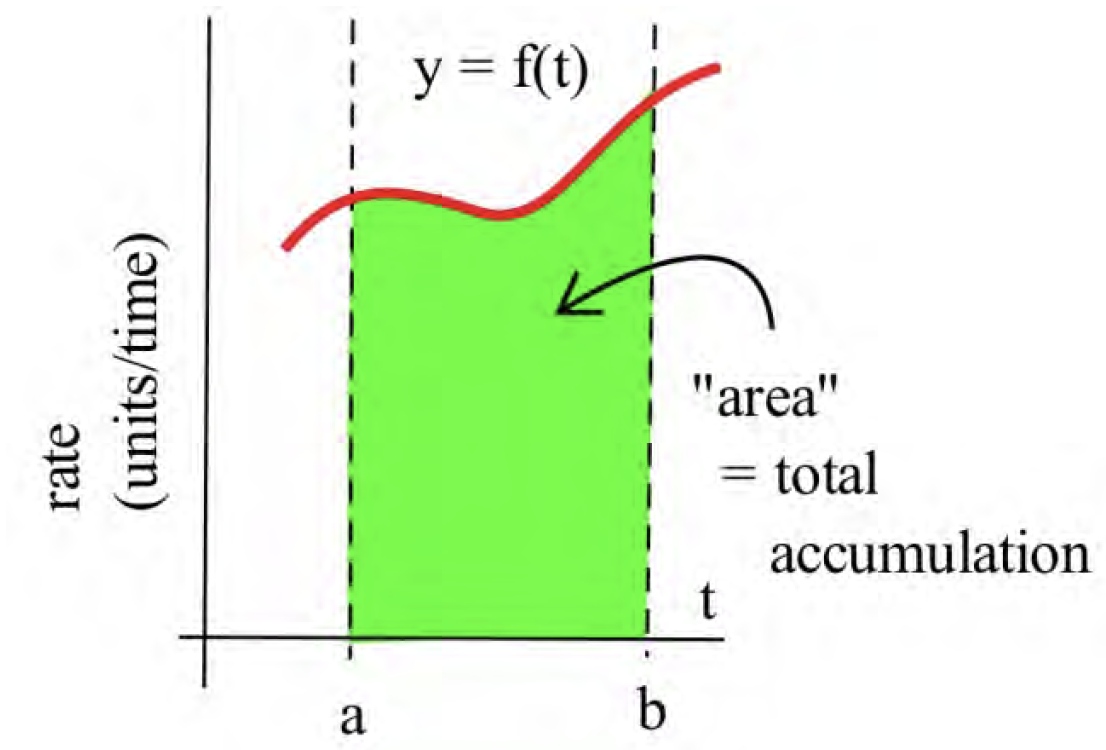
\includegraphics[scale=0.35]{images/defIntgArea/rate_TotalAmt.png}
\caption{ }
\label{fig:rate_TotalAmt}
\end{wrapfigure}

\noindent For functions representing other \textbf{rates} such as the production of a factory (bicycles per day), or the flow of water in a river (gallons per minute) or traffic over a bridge (cars per minute), or the spread of a disease (newly sick people per week), the area will still represent the \textbf{total} amount of something.\\

\begin{wrapfigure}[12]{r}{0.5\textwidth}

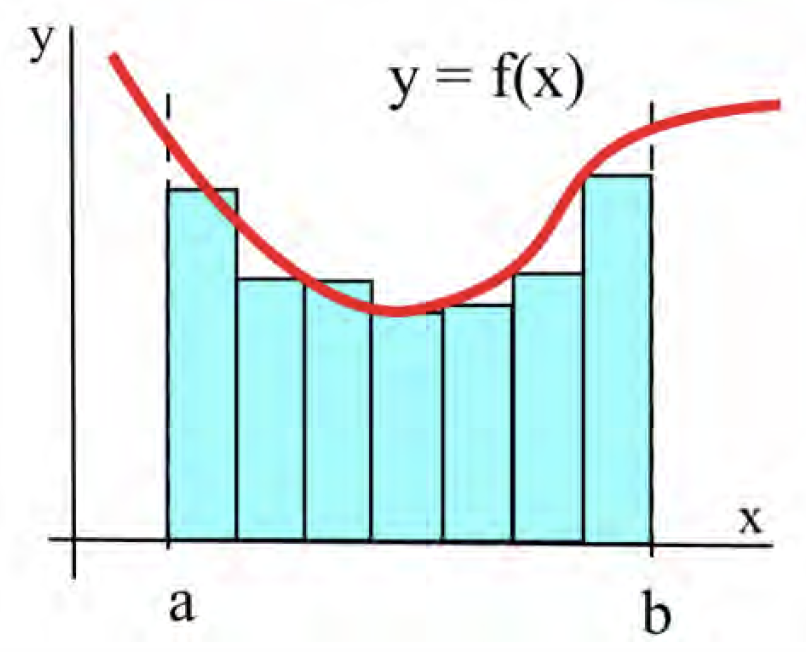
\includegraphics[scale=0.4]{images/defIntgArea/RiemannSum.png}
\caption{ }
\label{fig:RiemannSum}
\end{wrapfigure}
\noindent Suppose we want to calculate the area between the graph of a positive function $f$ and the $x$–axis on the interval $[a, b]$ (graphed on figure \ref{fig:RiemannSum}). The \textbf{Riemann Sum method} is to build several rectangles with bases on the interval $[a, b]$ and sides that reach up to the graph of $f$. Then the areas of the rectangles can be calculated and added together to get a number called a Riemann Sum of $f$ on $[a, b]$. The area of the region formed by the rectangles is an \textbf{approximation} of the area we want.\\

\noindent These sums of areas of rectangles are called \textbf{Riemann sums}. You may see a shorthand notation used when people talk about sums. We won’t use it much in this class, but you should know what it means.
\newpage
\begin{tcolorbox}[title = {Riemann Sum}]
A \textbf{Riemann sum} for a function $f(x)$ over an interval $[a, b]$ is a sum of areas of rectangles that approximates the area under the curve. Start by dividing the interval [a, b] into n subintervals; each subinterval will be the base of one rectangle. We usually make all the rectangles the same width $\triangle x$. The height of each rectangle comes from the function evaluated at some point in its sub interval. Then the \textbf{Riemann sum} is:
\vspace*{-0.5cm}
\begin{equation}\label{eq:riemann}
    f(x_1)\triangle x+f(x_2)\triangle x+f(x_3)\triangle x+...+f(x_n)\triangle x
\end{equation}
\textbf{Sigma Notation}: The upper-case Greek letter Sigma $\sum$ is used to stand for Sum. Sigma notation is a way to compactly represent a sum of many similar terms. Using the Sigma notation, the Riemann sum can be written
\vspace*{-0.5cm}
\begin{equation}\label{eq:riemannSigma}
    \sum_{i=1}^{n} f(x_i)\triangle x 
\end{equation}
This is read alound as " the sum as $i=1$ to $n$ of $f$ of $x$ sub $i$ Delta $x$." The "$i$" is a counter, like you might have seen in a programming class.
\end{tcolorbox}

\begin{tcolorbox}[title = {Formal Definition of Definite Integral and Riemann Sum}]
\noindent If $f(x)$ is continuous and  over an interval $[a,b]$, and the function $F(x)$ is any antiderivative of $f(x)$ (that is, $F'(x)=f(x)$, then 
\begin{equation}\label{defIntgRiemann}
    \int_{a}^{b} f(x) dx=\lim_{x\to\infty}\sum_{i=1}^{n} f(x_i)\triangle x 
\end{equation}
\textbf{Practical Definition: }The definite integral can be approximated with a \emph{Riemann sum} (dividing the area into rectangles where the height of each rectangle comes from the function, computing the area of each rectangle, and adding them up). The more rectangles you use, the narrower the rectangles are, the better your approximation will be.
\end{tcolorbox}


\noindent Since finding definite integrals using limits of \emph{Riemann sums} is cumbersome and is beyond the scope of this course, we will use the techniques of integration we learned in the previous sections that are developed from the \textbf{Fundamental Theorem of Calculus, Part 2 } or also known as the \textbf{Evaluation Theorem} .

\begin{tcolorbox}[title = {Review: Calculating Definite Integral using The Evaluation Theorem}]
\noindent If $f(x)$ is continuous and  over an interval $[a,b]$, and the function $F(x)$ is any antiderivative of $f(x)$ (that is, $F'(x)=f(x)$, then 
\begin{equation}\label{eq:evaluationTheorem}
\int_{a}^{b} f(x) dx = F(b)-F(a)    
\end{equation}

\noindent We often see the notation $F(x)\big|_{a}^{b}$ to denote the expression $F(b)-F(a)$. We use this vertical bar and associated \textbf{limits of integration} $a$ and $b$ to indicate that we should evaluate the function $F(x)$ at the \textbf{upper limit} $b$, and subtract the value of the function $F(x)$ evaluated at the \textbf{lower limit} $a$.\\

\end{tcolorbox}
\begin{comment}
\begin{tcolorbox}[title = {The Definite Integral and Signed Area}]
\noindent The \textbf{definite integral} of a function $f(x)$ over an interval $[a, b]$ is the \textbf{signed area}
between $f$, the $x$-axis, $x = a$ and $x = b$.\\

\end{tcolorbox}
\end{comment}
\noindent Before introducing the formal definition of the definite integral as \textbf{Net Signed Area} and as \textbf{Total Area}, let's consider the following application of velocity function to get some basic intuition of the difference between these two types of area. \\

\noindent One application of the definite integral is finding displacement when given a velocity function. If $v(t)$ represents the velocity of an object as a function of time, then the area under the curve tells us how far the object is from its original position. In the context of displacement, \textbf{net signed area} allows us to take \emph{direction} into account. If a car travels straight \emph{north} at a speed of $v(t)=60$ mph for 2 hours, it is 120 miles north of its starting position. using integral notation, we have 
\begin{equation}
    \int_0^2 60 dt=60t\big|_{0}^{2}=(60\cdot 2)-(60\cdot 0)=120
\end{equation}
\noindent If the car then turns around and travels \emph{south} at a speed of $v(t)=-40$ mph for 3 hours, it is 120 miles \emph{south} of its the turning-around point. Notice that the velocity now has a negative sign since the car is heading to the opposite direction (i.e. heading south instead of heading north). Again, using integral notation, we have
\begin{equation}
    \int_2^5 -40 dt=-40t\big|_{2}^{5}=(-40)(5)-(-40)(2)=-200+80=-120
\end{equation}
\noindent As a result, the car will be back at the starting position. In this case the displacement is zero or the \textbf{net signed area} is zero as shown in equation \ref{eq:netAreaCar1} and in figure \ref{fig:netAreaCar}
\begin{equation}\label{eq:netAreaCar1}
  \int_0^2 60 dt+\int_2^5 -40 dt=120-120=0
\end{equation}

\noindent Suppose we want to know how far the car travels overall, regardless of direction. In this case, we want to know the area
between the curve and the x-axis, regardless of whether that area is above or below the axis. This is called the \textbf{total area}.\\

\noindent Graphically, it is easiest to think of calculating \textbf{total area} by adding the areas above the axis and the areas below the axis
(rather than subtracting the areas below the axis, as we did with net signed area). To accomplish this mathematically, we use
the absolute value function. Thus, the total distance traveled by the car is 240 miles. Using integral notation, we have
\begin{equation}\label{eq:netAreaCar2}
    \int_0^2 |60| dt+\int_2^5 |-40| dt=120+120=240
\end{equation}

\noindent Bringing these ideas together formally, we state the following definitions.
\begin{tcolorbox}[title = {Net Signed Area vs. Total Area}]
Let $f(x)$ be an integrable function defined on an interval $[a,b]$. Let $A_1$ represent the area between $f(x)$ and the $x-$axis that lies \emph{above} the axis and let $A_2$ represent the are between $f(x)$ and the $x-$axis that lies \emph{below} the axis. Then, the \textbf{net signed area} between $f(x)$ and the $x-$axis is given by
\begin{equation*}
    \int_a^b f(x) dx=A_1-A_2
\end{equation*}
The \textbf{total area} between $f(x)$ and the $x-$axis is given by
\begin{equation*}
    \int_a^b \bm{|}f(x)\bm{|} dx=A_1+A_2
\end{equation*}
\end{tcolorbox}
%\vspace*{-0.6cm}
\newpage
\begin{figure}[h!]
    \centering
    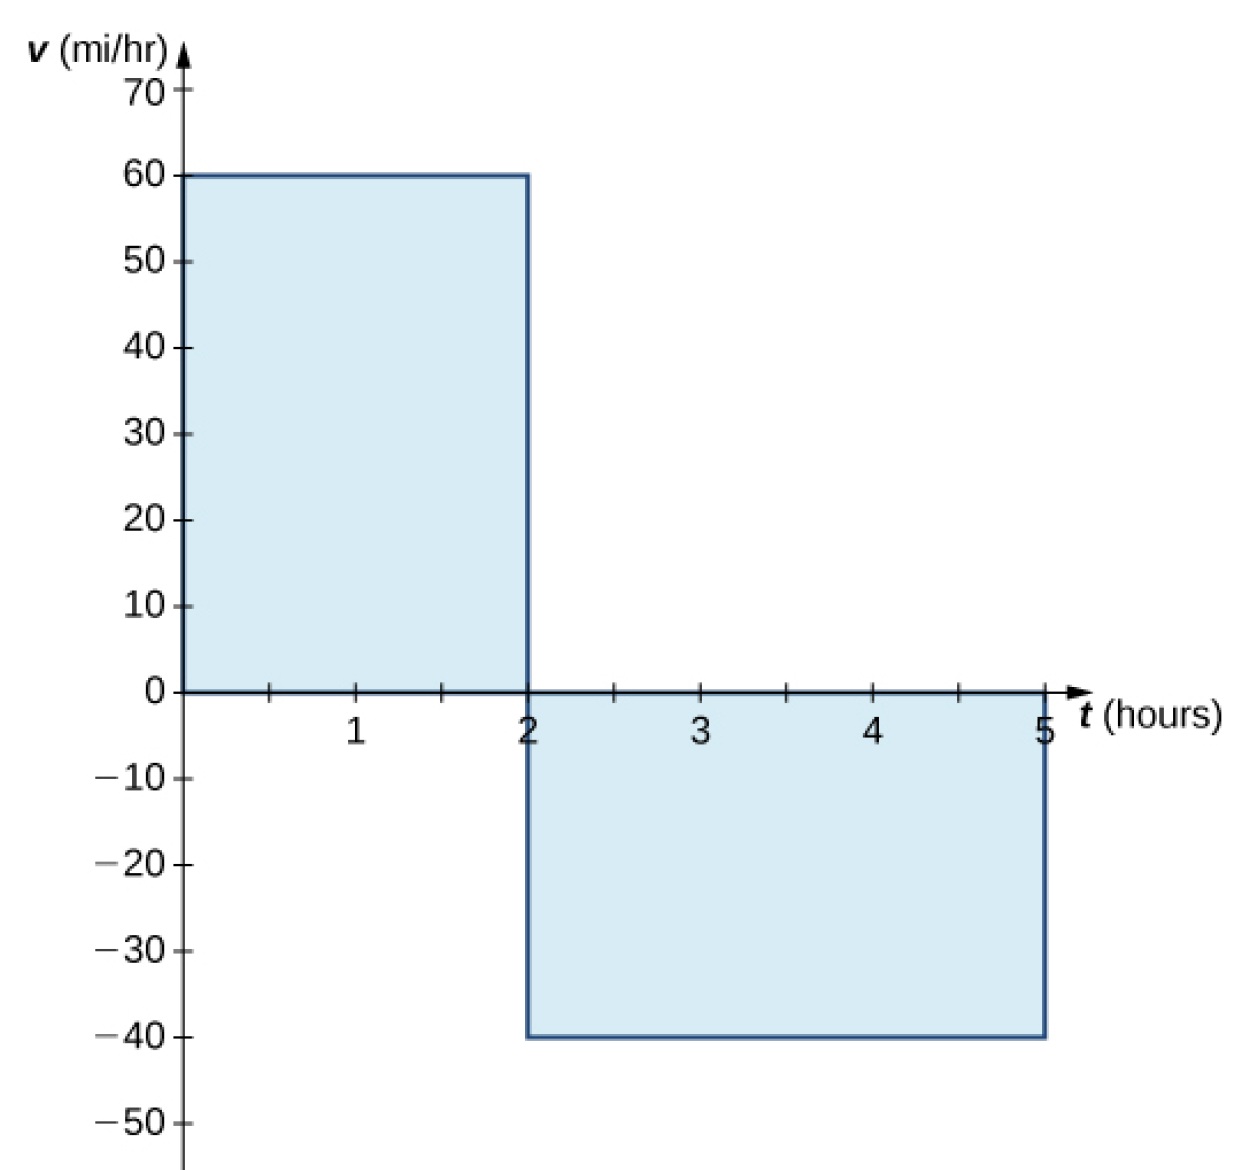
\includegraphics[scale=0.4 ]{images/defIntgArea/carVelocity.png}
    \caption{The area above the axis and the area below the axis are equal, so the \textbf{net signed area} is zero but the \textbf{total area} is 240.}
    \label{fig:netAreaCar}
\end{figure}
%\vspace{-0.5cm}

\begin{tcolorbox}[title={Review: Absolute Value Function}]
For $f(x)\ge 0$ (the graph of $f$ lies \emph{above} the $x-$axis),
\begin{equation}
   \left\bm{|}f(x)\right\bm{|}=f(x)
\end{equation}
For $f(x)< 0$ (the graph of $f$ lies \emph{below} the $x-$axis),
\begin{equation}
   \left\bm{|}f(x)\right\bm{|}=-f(x)
\end{equation}
\end{tcolorbox}
\vspace{1cm}
\begin{tcolorbox}[title = {Rule: Some Useful Properties of the Definite Integral}]
\begin{equation}
    \int_a^b cf(x)\,dx=c\int_a^b f(x)\, dx
\end{equation}
for constant $c$. The integral of the product of a constant and a function is equal to the constant multiplied bythe integral of the function.
\begin{equation}
    \int_a^b f(x)\,dx=\int_a^c f(x)\, dx+\int_c^b f(x)\, dx
\end{equation}
Although this formula normally applies when $c$ is between $a$ and $b$, the formula holds for all values of $a$, $b$, and $c$, provided $f(x)$ is integrable on the largest interval.\\

\emph{For more rules, see} \cite{openstax}\footnotemark[1].
\end{tcolorbox}
\footnotetext[1]{Available free to download from \url{https://openstax.org/details/books/calculus-volume-1} .}



\newpage
%%%Examples%%%
\begin{example}
\underline{Determine} and \underline{shade} the (total) area bounded by the $x-$axis and the graph of the function $f(x)=-x^2+3x$ on the interval from $x=0$ to $x=3$. The graph of $f$ is given below. 
\begin{figure}[h!]
        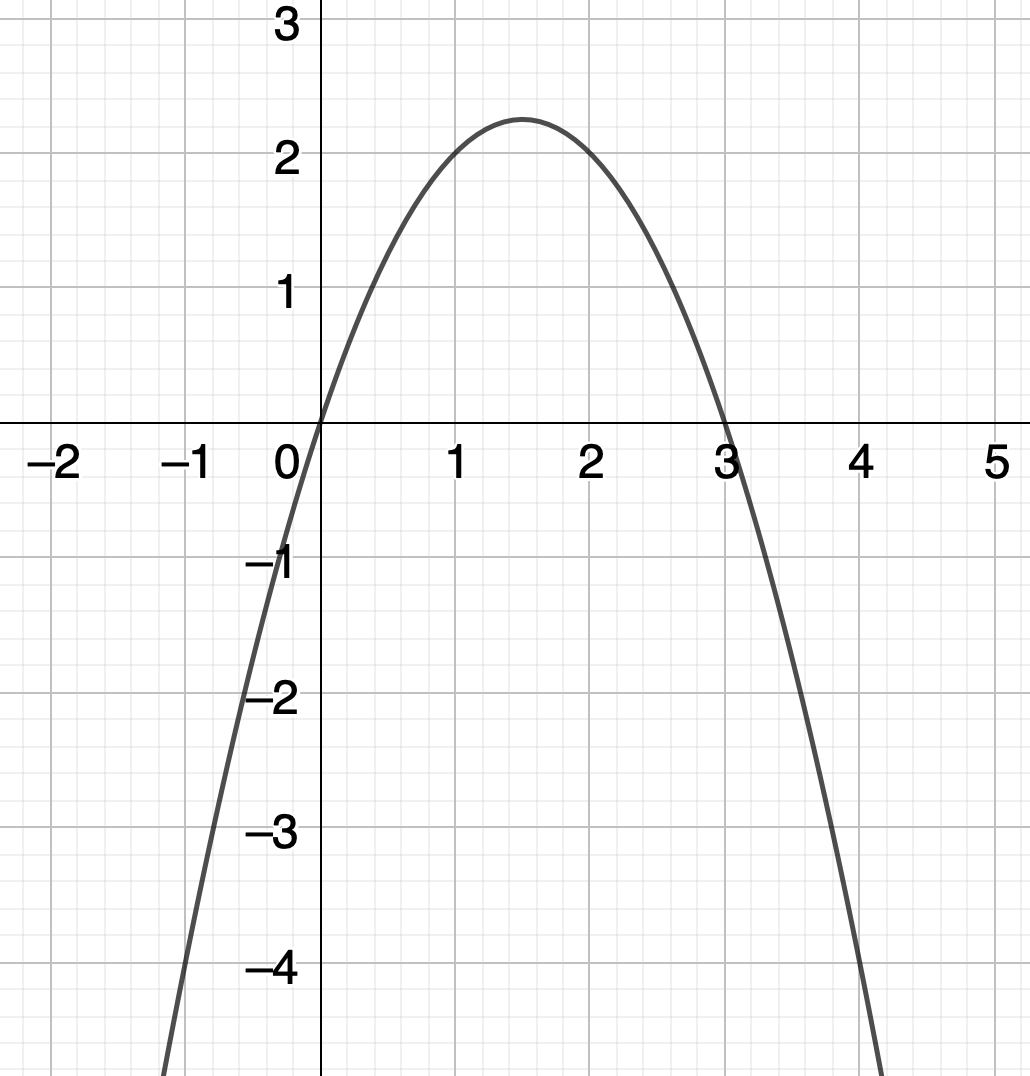
\includegraphics[width=0.25\textwidth,inner]{images/defIntgArea/areaEx1.png}
        \captionsetup{justification=justified, singlelinecheck=false}
        \label{fig:areaEx1}
\end{figure}
    %%short answer
    \begin{sol}
    $\displaystyle\int_0^3 \bm{|}f(x)\bm{|}\,dx=\int_0^3 f(x)\,dx=\left.-\frac{1}{3}x^3+\frac{3}{2}x^2\right|_{0}^{3}= \frac{9}{2}=4.5$. Note that $\left|f(x)\right|=f(x)$ since $f(x)\ge 0$ (the graph of $f$ is above the $x-$axis) on the interval $[0,3]$.
    \end{sol}
    %%solution
    \begin{solL}
    Complete solution here.....
    
    \end{solL}
    
\end{example}
\vspace*{\stretch{1.25}}

%%%%%%%%%%%%%%%%%%%%%%%%
%%%Examples%%%
\begin{example}
\underline{Determine} and \underline{shade} the (total) area bounded by the $x-$axis and the graph of the function $f(x)=3e^{\frac{1}{3}x}$ on the interval from $x=0$ to $x=3$. Give the exact form of the area, then a 2-decimal place approximation. The graph of $f$ is given below. 
\begin{figure}[h!]
        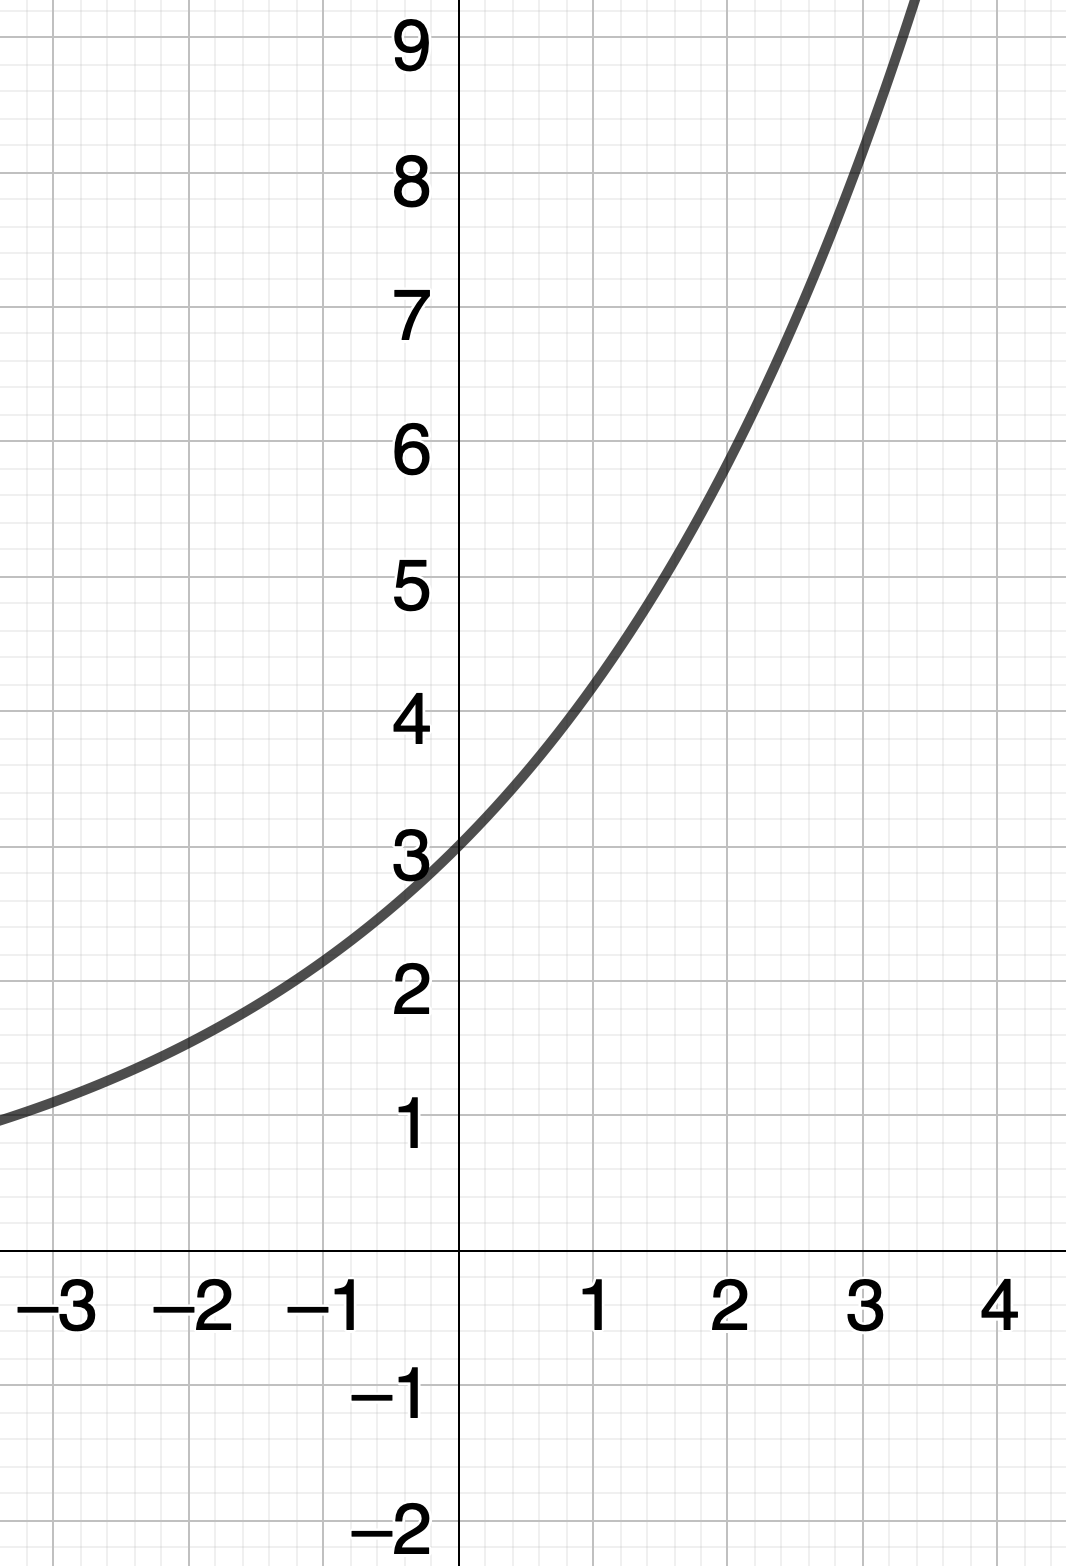
\includegraphics[width=0.2\textwidth,inner]{images/defIntgArea/areaEx2.png}
        \captionsetup{justification=justified, singlelinecheck=false}
        \label{fig:areaEx2}
\end{figure}

    %%short answer
    \begin{sol}
    $\displaystyle\int_0^3 \bm{|}f(x)\bm{|}\,dx=\int_0^3 f(x)\,dx=\left.9e^{\frac{1}{3}x}\right|_{0}^{3}=9e-9\approx 15.46$
    \end{sol}
    %%solution
    \begin{solL}
    Complete solution here.....
    
    \end{solL}
\end{example}
\vspace*{\stretch{1}}
\newpage
%%%Examples%%%
\begin{example}
Given the function $f(x)=x(x^2+1)^3$ and its graph given below, answer the following questions: 
\renewcommand{\labelenumi}{\textbf{(\alph{enumi})}}
\begin{enumerate}[leftmargin=*]
    \item \underline{Determine} and \underline{shade} the \textbf{(total) area} bounded by the $x-$axis and the graph of $f$ on the interval from $x=-1$ to $x=0$. 
    \item \underline{Determine} and \underline{shade} the \textbf{(total) area} bounded by the $x-$axis and the graph of $f$ on the interval from $x=0$ to $x=1$. 
     \item \underline{Determine} and \underline{shade} the \textbf{(total) area} bounded by the $x-$axis and the graph of $f$ on the interval from $x=-1$ to $x=1$. 
    \item Determine the \textbf{net signed area} bounded by the $x-$axis and the graph of $f$ on the interval from $x=0$ to $x=1$.
\end{enumerate}
 
\begin{figure}[h!]
        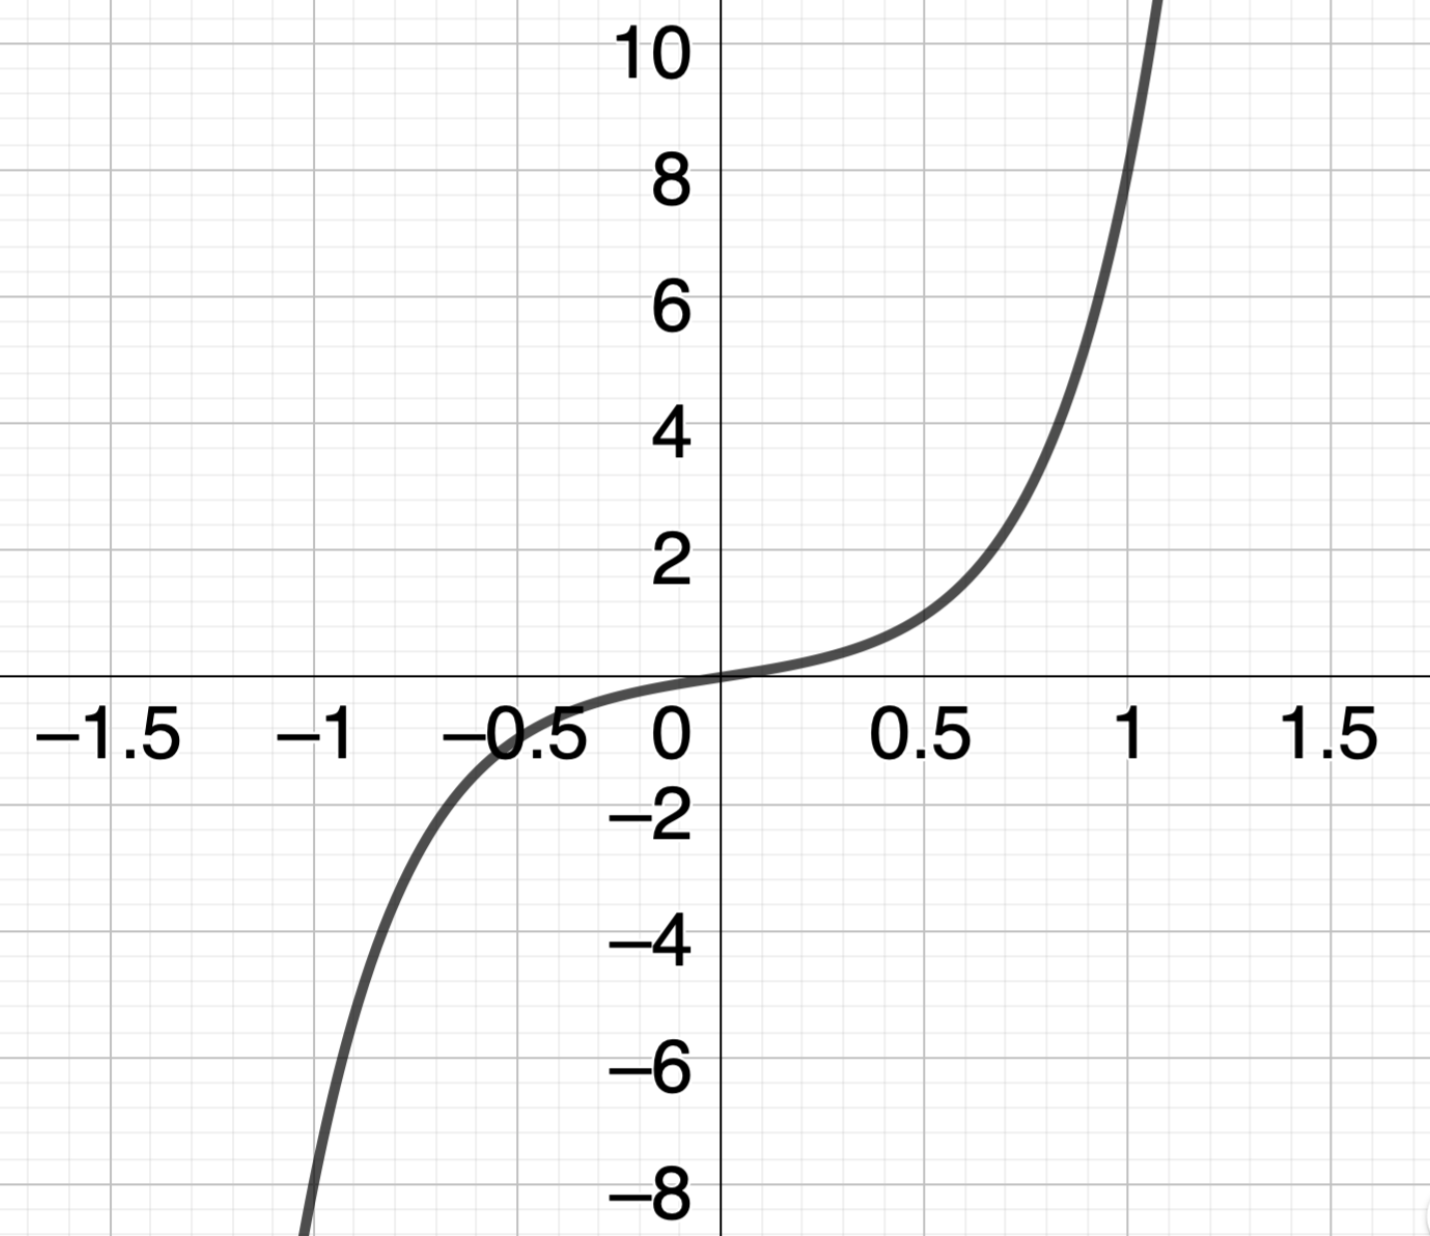
\includegraphics[width=0.4\textwidth,inner]{images/defIntgArea/areaEx3.png}
        \captionsetup{justification=justified, singlelinecheck=false}
        \label{fig:areaEx2}
\end{figure}

    %%short answer
    
    \begin{sol}
    \renewcommand{\labelenumi}{\textbf{(\alph{enumi})}}
    \begin{enumerate}[leftmargin=*]
        \item $\displaystyle\int_{-1}^0 \bm{|}f(x)\bm{|}\,dx=\int_{-1}^0 -f(x)\,dx=-\int_{-1}^0 f(x)\,dx=\left.-\frac{1}{8}(x^2+1)\right|_{-1}^{0}= \frac{15}{8}=1.875$. Note that $\left|f(x)\right|=-f(x)$ since $f(x)< 0$ (the graph of $f$ is below the $x-$axis) on the interval $[-1,0)$.
        \item $\displaystyle\int_0^1 \bm{|}f(x)\bm{|}\,dx=\int_0^1 f(x)\,dx=\left.\frac{1}{8}(x^2+1)\right|_0^1= \frac{15}{8}=1.875$. Note that $\left|f(x)\right|=f(x)$ since $f(x)\ge 0$ (the graph of $f$ is above the $x-$axis) on the interval $[0,1]$.
        \item $\displaystyle\int_{-1}^1 \bm{|}f(x)\bm{|}\,dx=\int_{-1}^0 \bm{|}f(x)\bm{|}\,dx+\int_0^1 \bm{|}f(x)\bm{|}\,dx=1.875+1.875=3.75$
        \item $\displaystyle\int_{-1}^1 f(x)\,dx=\int_{-1}^0 f(x)\,dx+\int_0^1 f(x)\,dx=-1.875+1.875=0$
    \end{enumerate}
    \end{sol}
    %%solution
    \begin{solL}
    Complete solution here.....
    
    \end{solL}
\end{example}
%%%Examples%%%
\newpage
\begin{example}
Given the function $f(x)=4x^3-4x^2$ and its graph given below, answer the following questions: 
\renewcommand{\labelenumi}{\textbf{(\alph{enumi})}}
\begin{enumerate}[leftmargin=*]
    \item \underline{Determine} and \underline{shade} the \textbf{(total) area} bounded by the $x-$axis and the graph of $f$ on the interval from $x=0$ to $x=2$. 
    \item Determine the \textbf{net signed area} bounded by the $x-$axis and the graph of $f$ on the interval from $x=0$ to $x=2$.
\end{enumerate}
 
\begin{figure}[h!]
        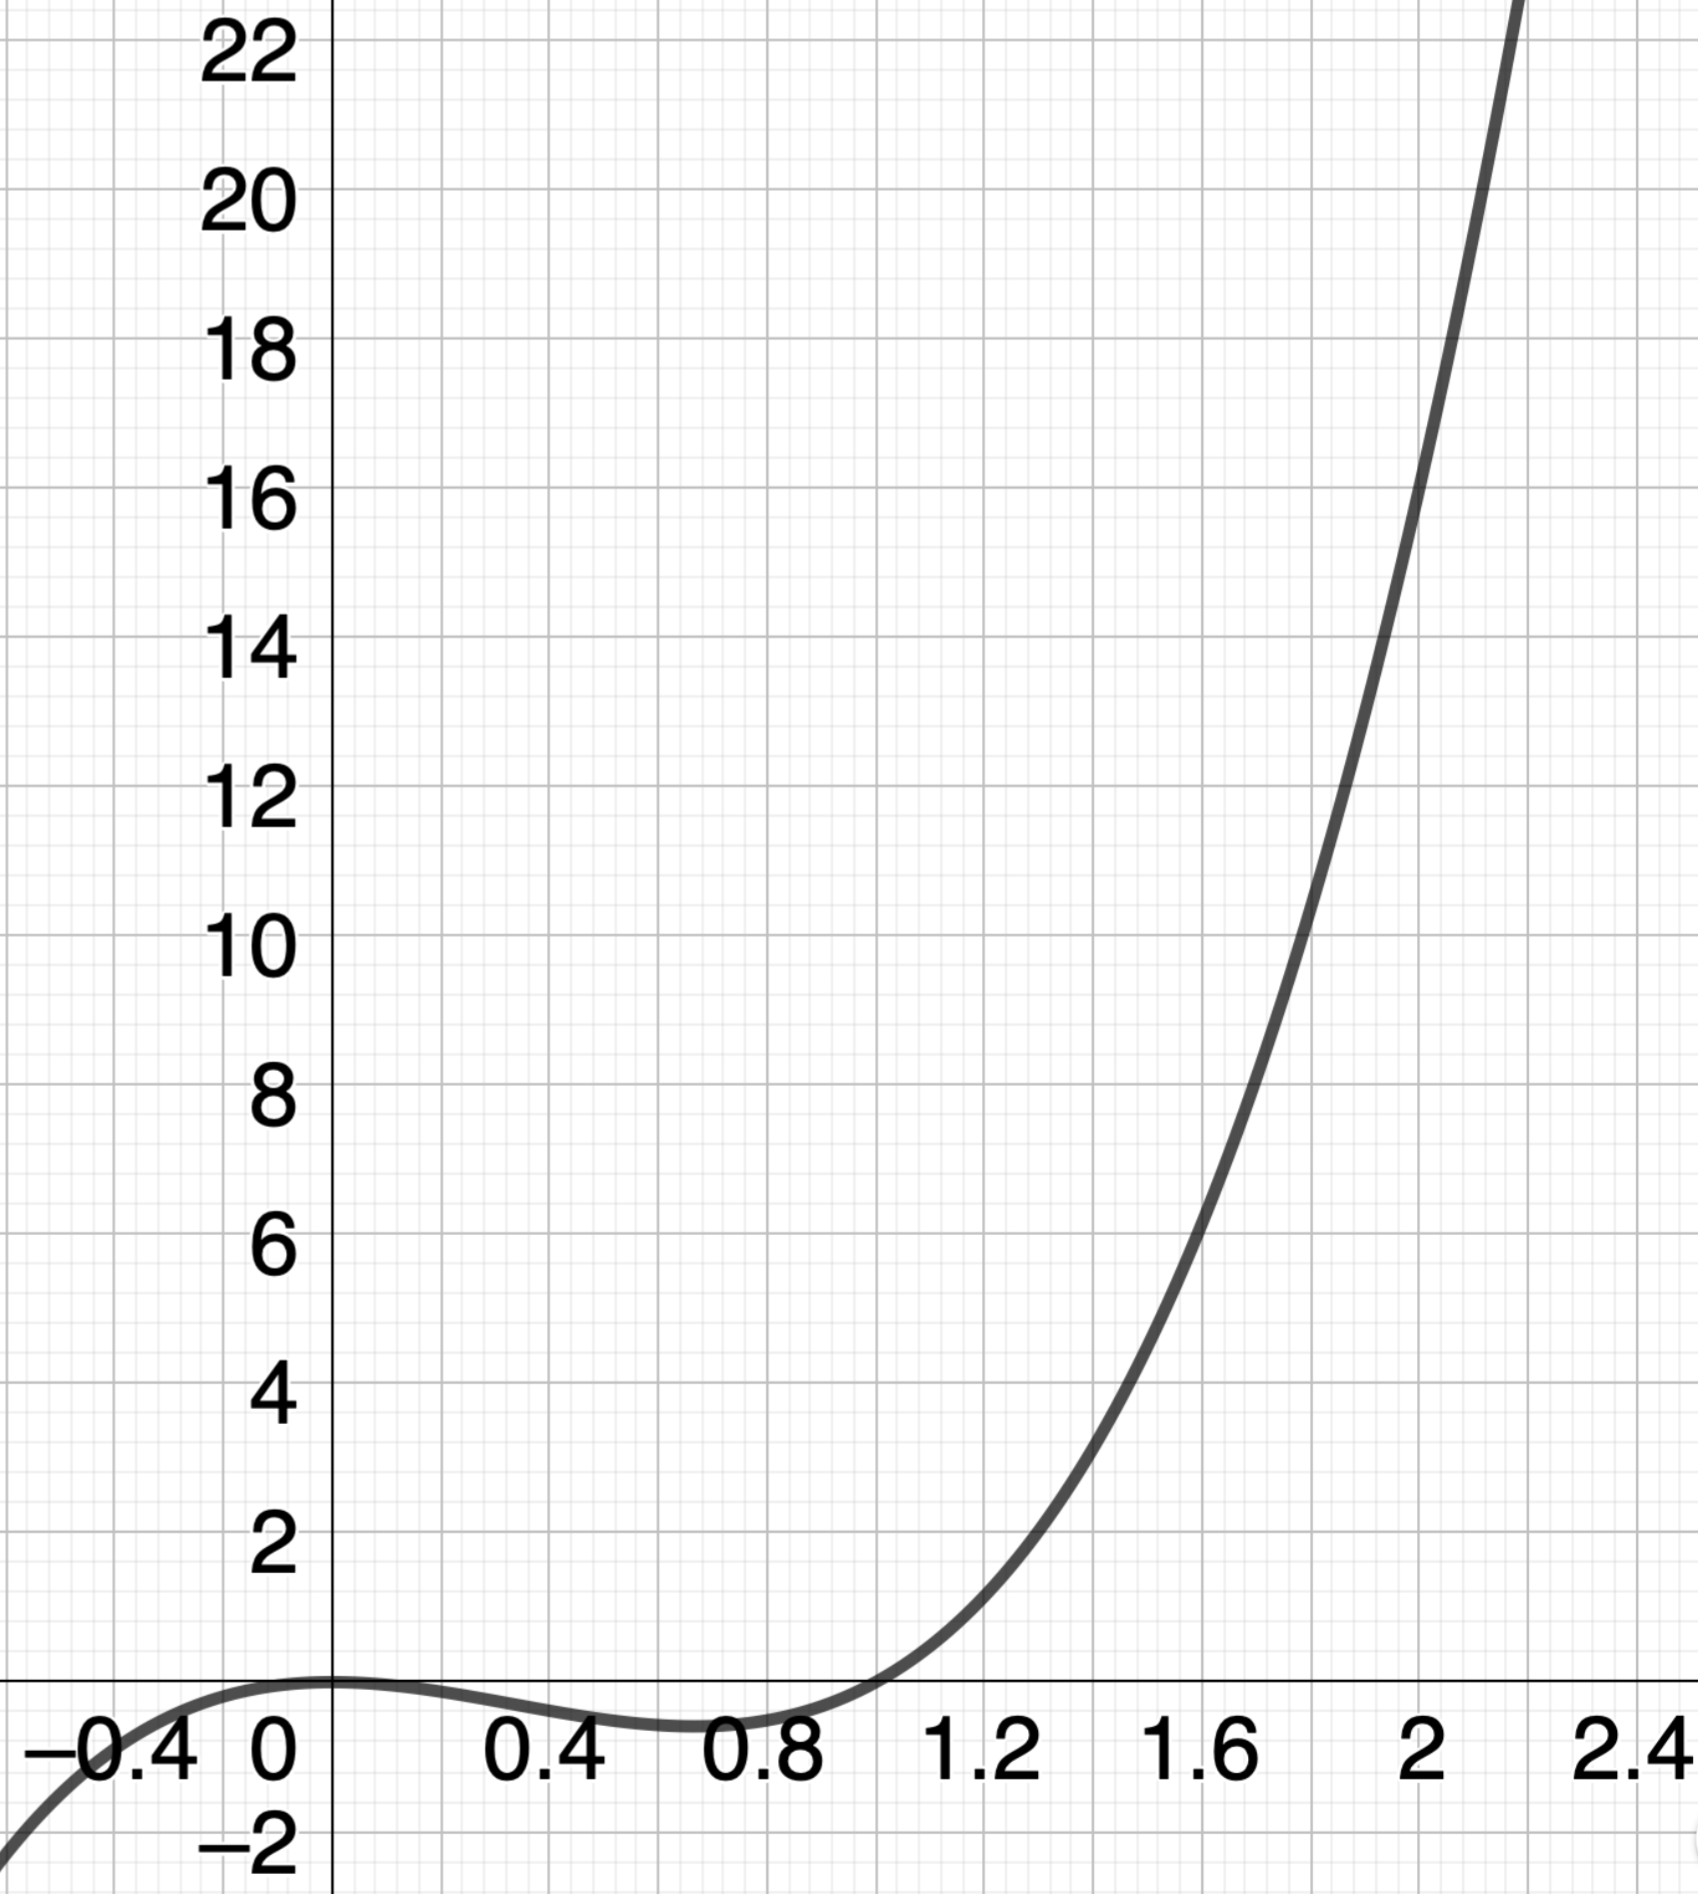
\includegraphics[width=0.5\textwidth,inner]{images/defIntgArea/areaEx4.png}
        \captionsetup{justification=justified, singlelinecheck=false}
        \label{fig:areaEx2}
\end{figure}

    %%short answer
    \begin{sol}
    \renewcommand{\labelenumi}{\textbf{(\alph{enumi})}}
    \begin{enumerate}[leftmargin=*]
    \item $\displaystyle\int_0^2 \bm{|}f(x)\bm{|}\,dx=\int_0^1 \bm{|}f(x)\bm{|}\,dx+\int_1^2 \bm{|}f(x)\bm{|}\,dx=\int_0^1 -f(x)\,dx+\int_1^2 f(x)\,dx=\left[-(x^4-\frac{4}{3}x^3)\right]_0^1+\left[x^4-\frac{4}{3}x^3\right]_1^2=\frac{1}{3}+\frac{17}{3}=6$
        \item $\displaystyle\int_0^2 f(x)\,dx=\int_0^1 f(x)\,dx+\int_1^2 f(x)\,dx=\left[x^4-\frac{4}{3}x^3\right]_0^1+\left[x^4-\frac{4}{3}x^3\right]_1^2=-\frac{1}{3}+\frac{17}{3}=\frac{16}{3}$
    \end{enumerate}
    \end{sol}
    %%solution
    \begin{solL}
    Complete solution here.....
    
    \end{solL}
\end{example}

%%%%%%%%%%%%End Examples%%%%%%%%%%%%%%%%%%

%%%%%%%%%%%%End Examples%%%%%%%%%%%%%%%%%%
%%%%%%%%%%%%%%%End Topic%%%%%%%%%%%%%%%%%%



%%%%%%%%%%%%%%%End Lesson%%%%%%%%%%%%%%%%%%
\Closesolutionfile{ans}
\Closesolutionfile{ansL}

%%%Short Answers to Examples%%%
%\newpage
\vspace*{\fill}

\subsection*{Short Answers to Examples}
%\vspace{-0.25cm}
%\begin{multicols}{2}
\input{ans22}
%\end{multicols}


